\chapter{Erasmus}
ERASMUS is the EU's flagship education and training program enabling 200 000 students to study and work abroad each year. In addition, it funds co-operation between higher education institutions across Europe. The program supports not only students, but also professors and business staffs who want to teach abroad, as well as helping university staff to receive training.

ERASMUS seeks to enhance the quality and reinforce the European dimension of higher education by encouraging transnational cooperation between universities, boo-sting European mobility and improving the transparency and full academic recognition of studies and qualifications throughout the Union.

\begin{figure}[!htbp]
\centering
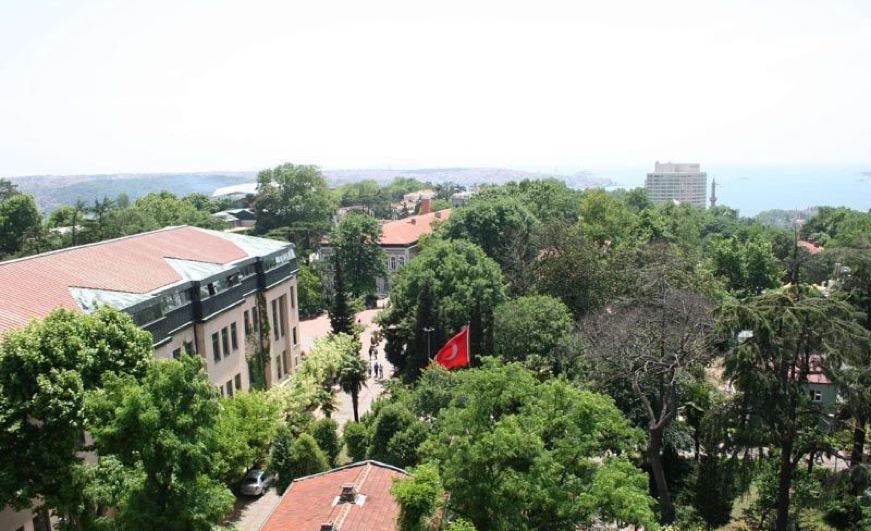
\includegraphics[width=\textwidth]{projectChapters/images/Picture1.png}
\caption{Landscape design of Yıldız Technical University}
\label{fig:ornek3}
\end{figure}

ERASMUS consists of many different activities; student and teacher exchanges, joint development of study program (Curriculum Development), international intensive programs, thematic networks between departments and faculties across Europe, language courses (EILC), European credit transfer system (ECTS).

ERASMUS action is targeted at higher education institutions and their students and staff in all 27 Member States of the European Union, the three countries of the European Economic Area (Iceland, Liechtenstein and Norway), and Turkey.

\begin{table}[!ht]
\caption{Erasmus country codes for different national agencies according to the type of the countries}
\centering
\begin{tabular}{|c|c|c|c|c|c|}
\hline
\textbf{No.} & \textbf{\begin{tabular}[c]{@{}c@{}}National\\ Agencies\end{tabular}}   & \textbf{\begin{tabular}[c]{@{}c@{}}Erasmus\\ Code\end{tabular}} & \textbf{\begin{tabular}[c]{@{}c@{}}ISO\\ Code\end{tabular}} & \textbf{\begin{tabular}[c]{@{}c@{}}NA \\ Identifier\end{tabular}} & \textbf{\begin{tabular}[c]{@{}c@{}}Type of\\ Country\end{tabular}} \\ \hline
1            & Austria                                                                & A                                                               & AT                                                          & AT                                                                & EU                                                                 \\ \hline
2            & \begin{tabular}[c]{@{}c@{}}Belgium\\ (Flemish\\ speaking)\end{tabular} & B                                                               & BE                                                          & BEFL                                                              & EU                                                                 \\ \hline
3            & \begin{tabular}[c]{@{}c@{}}Belgium\\ (French\\ speaking)\end{tabular}  & B                                                               & BE                                                          & BEFR                                                              & EU                                                                 \\ \hline
4            & Bulgaria                                                               & BG                                                              & BG                                                          & BG                                                                & Candidate                                                          \\ \hline
5            & \begin{tabular}[c]{@{}c@{}}Czech\\ Republic\end{tabular}               & CZ                                                              & CZ                                                          & CZ                                                                & EU                                                                 \\ \hline
6            & Cyprus                                                                 & CY                                                              & CY                                                          & CY                                                                & EU                                                                 \\ \hline
7            & Denmark                                                                & DK                                                              & DK                                                          & DK                                                                & EU                                                                 \\ \hline
8            & Estonia                                                                & EE                                                              & EE                                                          & EE                                                                & EU                                                                 \\ \hline
9            & Germany                                                                & D                                                               & DE                                                          & DE                                                                & EU                                                                 \\ \hline
10           & Spain                                                                  & E                                                               & ES                                                          & ES                                                                & EU                                                                 \\ \hline
11           & Finland                                                                & SF                                                              & FI                                                          & FI                                                                & EU                                                                 \\ \hline
12           & France                                                                 & F                                                               & FR                                                          & FR                                                                & EU                                                                 \\ \hline
13           & Greece                                                                 & G                                                               & GR                                                          & GR                                                                & EU                                                                 \\ \hline
14           & Hungary                                                                & HU                                                              & HU                                                          & HU                                                                & EU                                                                 \\ \hline
15           & Iceland                                                                & IS                                                              & IS                                                          & IS                                                                & EEA                                                                \\ \hline
16           & Ireland                                                                & IRL                                                             & IE                                                          & IE                                                                & EU                                                                 \\ \hline
17           & Italy                                                                  & I                                                               & IT                                                          & IT                                                                & EU                                                                 \\ \hline
18           & Latvia                                                                 & LV                                                              & LV                                                          & LV                                                                & EU                                                                 \\ \hline
19           & Liechtenstein                                                          & FL                                                              & LI                                                          & LI                                                                & EEA                                                                \\ \hline
20           & Lithuania                                                              & LT                                                              & LT                                                          & LT                                                                & EU                                                                 \\ \hline
21           & Luxembourg                                                             & LUX                                                             & LU                                                          & LU                                                                & EU                                                                 \\ \hline
22           & Malta                                                                  & MT                                                              & MT                                                          & MT                                                                & EU                                                                 \\ \hline
23           & Netherlands                                                            & NL                                                              & NL                                                          & NL                                                                & EU                                                                 \\ \hline
24           & Norway                                                                 & N                                                               & NO                                                          & NO                                                                & EEA                                                                \\ \hline
25           & Poland                                                                 & PL                                                              & PL                                                          & PL                                                                & EU                                                                 \\ \hline
26           & Portugal                                                               & P                                                               & PT                                                          & PT                                                                & EU                                                                 \\ \hline
27           & Romania                                                                & RO                                                              & RO                                                          & RO                                                                & Candidate                                                          \\ \hline
28           & \begin{tabular}[c]{@{}c@{}}Slovak\\ Republic\end{tabular}              & SK                                                              & SK                                                          & SK                                                                & EU                                                                 \\ \hline
29           & Slovenia                                                               & SI                                                              & SI                                                          & SI                                                                & EU                                                                 \\ \hline
30           & Sweden                                                                 & S                                                               & SE                                                          & SE                                                                & EU                                                                 \\ \hline
\end{tabular}
\label{tab:ornek1}
\end{table}


\section{Application Procedure}
You are expected to attach the following documents to the online application module.

\begin{itemize}
%\setlength{\itemsep}{0pt}
\item Application form
\item Learning agreement
\item Dormitory request form 
\item Signed documents
\item ID Card
\end{itemize}

\begin{figure}[!htbp]
\centering
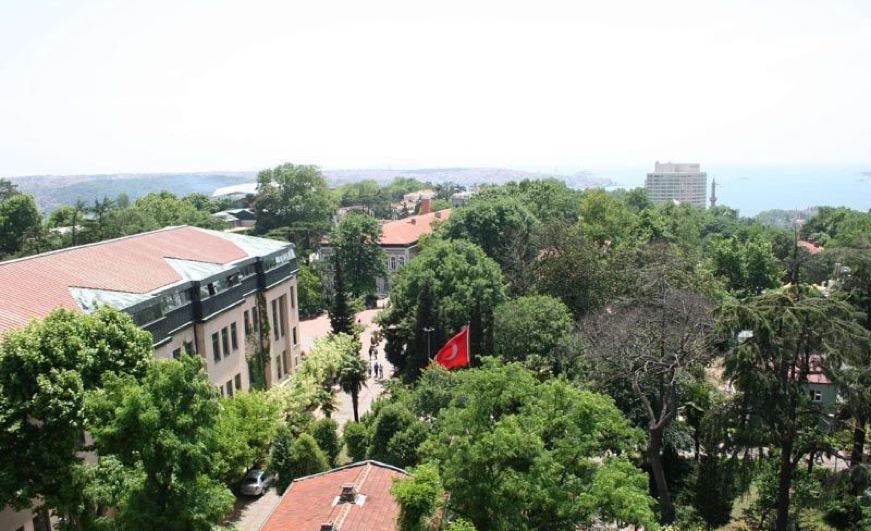
\includegraphics[width=\textwidth]{projectChapters/images/Picture1.png}
\caption{Landscape design of Yıldız Technical University}
\label{fig:ornek4}
\end{figure}

\section{Money Exchange}
The most convenient way to get money  in Turkey is by using your home bank ATM/ cash card or a credit card in a Turkish ATM/ bancomat/ cash machine.

\begin{table}[!ht]
\caption{Area codes for different subjects}
\centering
\begin{tabular}{|c|c|}
\hline
\textbf{Area Code} & \textbf{Subject}      \\ \hline
1                  & Agricultural sciences \\ \hline
2                  & Culture               \\ \hline
3                  & Economics             \\ \hline
4                  & Technology            \\ \hline
5                  & Horticulture          \\ \hline
6                  & Fisheries             \\ \hline
7                  & Forestry              \\ \hline
8                  & Animal                \\ \hline
9                  & Tropical Agriculture  \\ \hline
10                 & Others                \\ \hline
\end{tabular}
\end{table}

But if you want to exchange cash, plenty of places will do it for you. Currency Exchange Offices  are found in tourist and market areas. They offer better exchange rates than most banks, and may or may not charge a commission. Offices in market areas tend to offer better exchange rates than those in tourist areas. Shop around for the best rate and the lowest (or no) commission.

\section{After a Car Accident}
The following is a step-by-step guide on what to do if you are involved in a traffic accident in Turkey.
From 1 April 2008 it is no longer necessary to call the police to the scene of an accident in the following circumstances:\cite{guo2004learning}

\begin{itemize}
\item When - the accident involves two or more vehicles
\item Where there is only material damage to vehicles
\item When no one is injured or killed
\end{itemize}

Where all concerned parties agree to the cause and who is liable for the accident and providing each driver completes the correct form and all parties involved sign each form, including witnesses if any. 

You should then submit the form to your insurance company who will use the form in conjunction with the other insurance companies concerned to settle liability. (For more details about how to access the form and instructions how to complete the form, please look at the end of this document.) \cite{van2007experimental}

If agreement cannot be reached, you should immediately call 155 for Traffic Police assistance and follow the guide below:
Do Not Move Your Vehicle from the point of impact unless invited to do so by the traffic police or gendarme.

It is not advisable to accept an offer of financial settlement from the other parties involved. Wait for the police to arrive.
Once the police arrive, you will be breathalyses and asked to produce your driving license and logbook. A preliminary report of the accident will be compiled by the police at the scene of the accident. Only when this report has been made, should you move your vehicle.  It can take half an hour for the police to arrive at the scene of an accident. Do not move your vehicle.

It is essential to obtain the result of the breathalyzer test and the official police report in order to make a successful insurance claim. You will be asked to collect this within three days from the District Police Station.

\begin{figure}[!htbp]
\centering
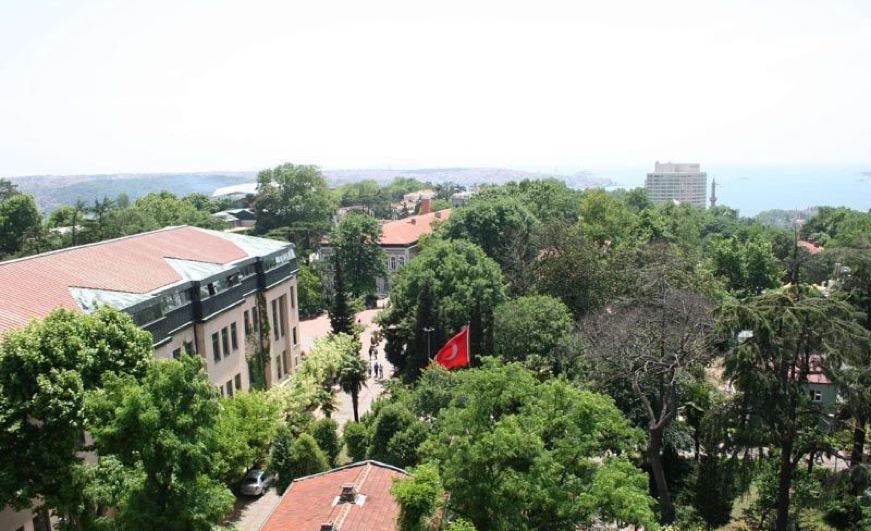
\includegraphics[width=\textwidth]{projectChapters/images/Picture1.png}
\caption{Landscape design of Yıldız Technical University}
\label{fig:ornek5}
\end{figure}

This leaflet has been prepared by the British Embassy in Ankara for the convenience of enquirers.  Although all care has not been taken in its production, neither Her Majesty's Government nor any Consular Official in the British Embassy in Ankara takes any responsibility for its precise accuracy or for the consequences of any action taken in accordance with its contents.